\documentclass[12pt, twoside]{article}
\RequirePackage{amssymb}
\usepackage{jmlda}
\newcommand{\hdir}{.}
\newtheorem{theorem}{Теорема}[section]
\newtheorem{lemma}[theorem]{Лемма}
\theoremstyle{definition}
\newtheorem{definition}[section]{Определение}
\graphicspath{ {./images/} }
\newcommand{\Tau}{\mathcal{T}}
\begin{document}

\title
    [Экспериментальное сравнение моделей планирования биохимического производства.] % краткое название; не нужно, если полное название влезает в~колонтитул
    {Экспериментальное сравнение моделей планирования биохимического производства.}
\author
    [В.\,В.~Пырэу, С.\,А.~Тренин] % список авторов (не более трех) для колонтитула; не нужен, если основной список влезает в колонтитул
    {В.\,В.~Пырэу, С.\,А.~Тренин} % основной список авторов, выводимый в оглавление
\email
    {kondratiukvitalik@gmail.com; s.trenin@gmail.com}
\abstract
    {Целью данной работы является исследование задачи оперативного планирования производства для биохимической промышленности. Анализируются различные постановки задачи составления расписания, учитывающие ограничения, приходящие из практики хранение промежуточных веществ, требования к работе производственных узлов и подготовка станков, например наладка и очистка между запусками. Рассматриваются модели смешанного целочисленного линейного программирования. Это означает, что задачи являются $\NP$-трудными. Основная трудность заключается в том, что при моделировании задач с схожим описанием модели могут сильно отличаться по сложности (числу переменных и ограничений), что негативно сказывается на процессе внедрения моделей в практику. Для решения этого вопроса проводится экспериментальный запуск моделей, разработанных для одной предметной области, в задачах из другой и интерпретация полученных результатов.
    
    
\bigskip
\noindent
\textbf{Ключевые слова}: \emph {planning; scheduling; MILP}
}

%данные поля заполняются редакцией журнала
\doi{}
\receivedRus{}
\receivedEng{}

\maketitle
\linenumbers

\section{Введение}
Основная решаемая задача --- планирование производства и создание расписаний в ограничениях, диктуемых особенностями ресурсов завода. Эта задача имеет практическое значение, так как производственные процессы усложняются, количество машин растёт, а, как следствие, растут размеры ограничений и имеющегося сырья. Это влечёт за собой то, что ручное создание расписаний и распределения сырья по машинам становится невозможным, а получаемые расписания --- слишком неэкономными. В работе \cite{reallife} приводится детальное описание и классификация постановок задач создания расписаний, а так же богатая классификация разработанных на момент методов моделирования. Основное поле для исследований --- это различные способы описать практические требования к расписанию так, чтобы математическая постановка задачи, как задачи оптимизации, было (1) простым и коротким и (2) позволяло найти оптимальное решение быстрее. Так как время работы является зависит не только от сложности постановки задачи, то основным критерием качества модели будет её сложность.

\begin{definition} \textbf{Модель} --- задача целочисленного линейного программирования в общей форме, описывающая практические требования. Значения переменных из допустимых решений задачи будут интерпретироваться как план производства. \textbf{Сложность модели} --- число её переменных и ограничений типа равенства и неравенства.
\end{definition}

В работах \cite{lpheuristic}, \cite{dairy}, \cite{discretetime}, \cite{hybridizing} описаны различные задачи из практики и предложены методы по их решению. Утверждается, что методы можно использовать перекрёстно, то есть не только на тех данных, для которых они предложены. Некоторые авторы, как например \cite{lpheuristic} предлагают модели, которые не гарантируют оптимальность полученных расписаний, однако гарантируют простоту самой модели. В работе описано, в при каких предположениях об описании процессов какие методы моделирования работают лучше, то есть создают модели с более простым описанием. 

\section{Описание имеющихся данных}
Так как авторы статьи поставили одной из своих целью собрать различные варианты постановок задач планирования из разных предметных областей, то в первую очередь необходимо эти задачи описать. Задача планирования состоит в том, что по описанию процесса необходимо указать, какие операции на каких машинах и с какими входными веществами нужно произвести, чтобы по имеющимся на складе прекурсорам получить заявленное количество продукта.

\begin{definition} \textbf{Прекурсор} --- вещество, имеющееся изначально на складе, из которого будут произведены все требуемые продукты. Также \textbf{промежуточным прекурсором} будем называть вещество, получаемое после некоторых этапов производства, но не требуемое для получения в финале.
\end{definition}

В описание задачи входят описания всех прекурсоров, описание производственных узлов --- сущностей, способных проводить реакции и описания рецептов приготовления промежуточных прекурсоров и финальных продуктов. Рецепт представляет собой описание одной операции: сколько нужно обрабатывать, на каком оборудовании и какие прекурсоры в какой пропорции, чтобы получить продукт. 

Вещества разрешается хранить на складе, который описывается максимальной вместимостью. Некоторые вещества, возможно, хранить нельзя вовсе.

В данной работе рассматривается только \textbf{пакетное производство}. В этом случае на узел подаётся пакет некоторого размера и обрабатывается. Продуктом является пакет вещества-продукта. Для каждого узла известен максимальный и минимальный размер пакета, который можно подать. Этот подход является альтернативным к \textbf{непрерывному производству}, где узлы оперируют с непрерывными потоками данных, но это требует другого подхода к созданию моделей, и поэтому не рассматривается для перекрёстного запуска моделей.

В зависимости от задачи, время обработки пакета может как зависеть, так и не зависеть от его размера. В работе описывается, какие модели способны работать с неравными временами обработки пакета, а какие нет и насколько изменится сложность модели.

Процессы, в зависимости от их структуры делятся на две большие группы: последовательные и сетевые.

\begin{definition} \textbf{Последовательный процесс} --- процесс, который может быть разделён на несколько стадий, упорядоченных во времени, и пакеты передаются на производство только от предыдущей стадии к следующей. В зависимости от числа стадий эти процессы делятся на \textbf{одноступенчатые} и \textbf{многоступенчатые}.
\end{definition}

Собственно, \textbf{сетевой} процесс --- это тот процесс, что не является последовательным. Как будет показано далее, сетевые процессы являются более общими, но и более сложными для моделирования. 

\begin{figure}[h]
\caption{Пример STN-диаграммы}
\centering
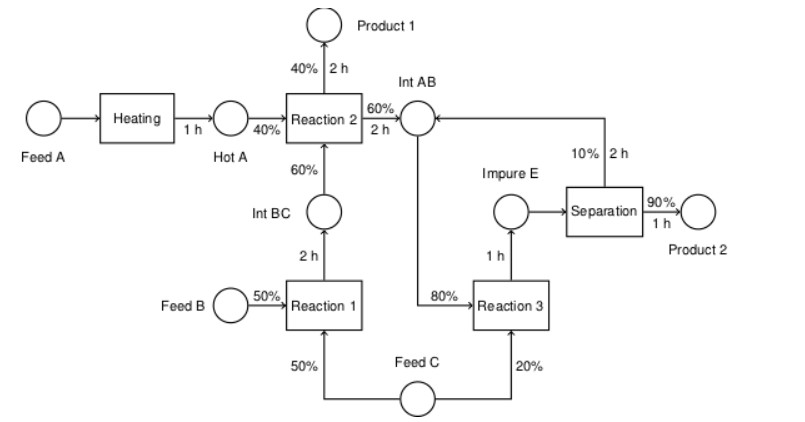
\includegraphics[width=1.0\textwidth]{пример процесса}
\label{fig:stn_exmp}
\end{figure}

Процессы (в особенности сетевые) удобно представлять себе в виде графов состояний (STN), впервые предложенных в работе \cite{stnoriginal}. Пример такого графа можно видеть на рисунке \ref{fig:stn_exmp}. Круглыми вершинами обозначаются склады веществ, прямоугольными --- задачи, а рёбрами --- поток материала (число над ребром --- процент вещества в пакете).

\begin{figure}[h]
\caption{Классификация процессов}
\centering
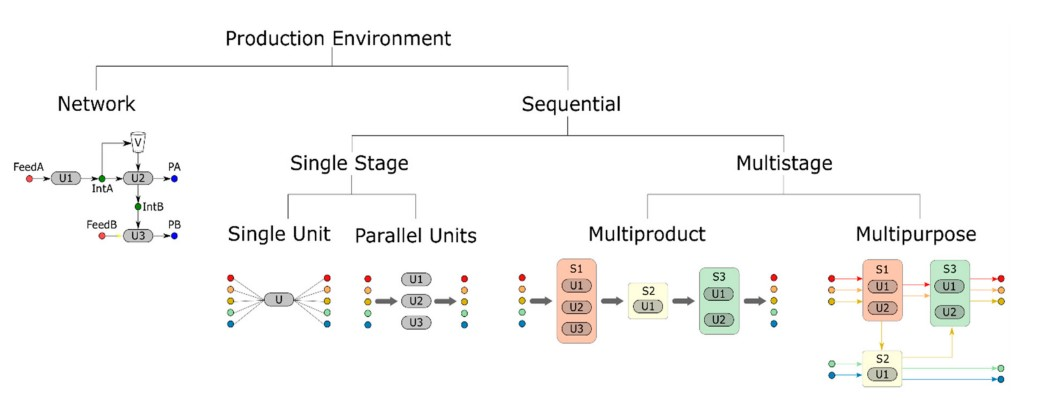
\includegraphics[width=1.0\textwidth]{классификация процессов}
\label{fig:clas_proc}
\end{figure}

Классификация \ref{fig:clas_proc} взята из \cite{reallife} где она является более подробной, но в этой статье параллелизм и наличие многих продуктов/прекурсоров являются параметрами модели. Основной вопрос состоит в том, как переход от последовательных процессов к сетевым изменяет модель и какие методы, изобретённые для последовательных моделей применимы к сетевым и наоборот. 

\section{Описание моделей}

Моделью в рамках данной работы будем называть задачу смешанного целочисленного линейного программирования в общей форме. На данном этапе необходимо закодировать решения, принимаемые системой составления расписаний в переменные, которые будут называться \textbf{решающими переменными}. Далее $T$ будет обозначать множество промежутков времени и переменные, с ним связанные. Другими большими латинскими буквами (с индексами) будут обозначаться непрерывные решающие переменные, малыми --- бинарные решающие переменные и индексы (в некоторых моделях бинарные переменные и являются своеобразными <<индексами>> того, что какое-то утверждение верно или нет). Также большими буквами будут обозначаться параметры модели и их множества. Строчные греческие буквы по умолчанию означают разные затраты, сопровождающие процесс (в моделях, где они присутствуют).

Опишем все обозначения, которые будут встречаться в эксперименте.

\begin{enumerate}
   \item Множества:
   \begin{itemize}
     \item $U$ --- множество производственных узлов. Индексы у этого множества означают:
     \begin{itemize}
     		\item $U_j$ --- узлы, способные производить задачу $j \in J$.
     \end{itemize}
     \item $P$ --- множество продуктов (как прекурсоры, так и те, что получаются в процессе реакций). Индексы у этого множества означают:
		\begin{itemize}
     		\item $P^{in}_j$ --- продукты, потребляемые задачей $j \in J$.
     		\item $P^{out}_j$ --- продукты, производимые задачей $j \in J$.
     		\item $P^{`}$ --- продукты, которые надо произвести к концу (заказ).
     \end{itemize}
     
     \item $T$ --- множество временных промежутков
     \item $J$ --- множество задач (задача есть производство некоторого вещества по его рецепту). Индексы у этого множества означают:
     \begin{itemize}
     		\item $J^{in}_p$ --- задачи, потребляющие продукт $p \in P$.
     		\item $J^{out}_p$ --- задачи, производящие продукт $p \in P$.
     		\item $J^{u}$ --- задачи, которые могут быть произведены на узле $u \in U$.
     \end{itemize}
   \end{itemize}
   \item Параметры:
   	\begin{itemize}
   		\item $B^{min}_u, B^{max}_u$ --- минимальный и максимальный размеры пакета для запуска узла $u \in U$.
   		\item $S^{max}_p$ --- максимальное количество продукта $p \in P$, которое может находиться на складе в любой момент времени.
   		\item $D_p$ --- внешние требования на производство продукта $p \in P^{`}$.
   		\item $I_p$ --- изначальное количество продукта $p \in P$ на складе.
   		\item $\Tau_{u, j}$ --- время работы задачи $j \in J$ на узле $u \in U$. По умолчанию считается, что время исполнения задачи не зависит от размера пакета. Будут рассмотренны случаи, в которых время может зависеть от размера пакета, в таком случае этот параметр значит <<время работы за килограмм входных веществ>>.
   		\item $\mathcal{Q}^{in}_{p, j}, \mathcal{Q}^{out}_{p, j}$ --- пропорции входного/выходного продукта $p \in P$ в пакете в рецепте задачи $j \in J$ в случае мультипотребления/мультипроизводства.
   		\item $\theta_{u}$ --- стоимость запуска оборудования $u \in U$ за единицу времени.
   		\item $\psi_{p}$ --- стоимость хранения продукта $p \in P$ на складе.
   		\item $\eta_{p, u}$ --- стоимость производства продукта $p \in P$ на узле $u \in U$ за килограмм.
   	\end{itemize}
\end{enumerate}

В моделях будет рассматриваться целевая функция <<Makespan>> --- общее время производства:
\begin{enumerate}
\item
\begin{equation}
\begin{gathered}
	min \: MS\\
	s.t.\\
	MS \leq T_{u, i} \: \forall u \in U, i \in \mathbb{N}
\end{gathered}
\end{equation}

Минимизация общего времени выполнения (makespan) при условиях, что оно больше, чем время окончания каждого запуска каждого узла --- $T_{u, i}$. В зависимости от представления времени в модели величина справа будет по-разному выражаться из переменных.

\end{enumerate}

\section{Вычислительный эксперимент}

Эксперимент состоит в том, что практическая задача будет закодирована разным способом в набор решающих переменных и ограничений и подана на вход COIN-OR Branch-and-Cut (CBC) алгоритму, а далее полученные значения будут интерпретированы и визуализированы в виде диаграмм Ганта. Цель эксперимента состоит в том, чтобы сравнить разные алгоритмы на разных данных и проинтерпретировать полученные результаты. Способ кодирования плана для солвера и интерпретации зависит от подхода к моделированию времени и является основным объектом исследований. Пример диаграммы Ганта можно найти в \cite{discretetime} и на рисунке \ref{fig:gannt_example}. Эта диаграмма соответствует некоторому плану для процесса \ref{fig:stn_exmp}. По оси Ox отложено время, а по оси oY --- производственные узлы. Прямоугольники --- это запуски задачи, а числа в них обозначают размер пакета для обработки. Такие диаграммы помогают визуально понять качество расписания и работы решающих алгоритмов. 

Основные метрики сравнения подходов к моделированию: количество переменных, количество ограничений, качество расписания, получаемого за ограниченное время, время, необходимое для получения оптимального расписания.

\begin{figure}[h]
\caption{Пример диаграммы Ганта}
\centering
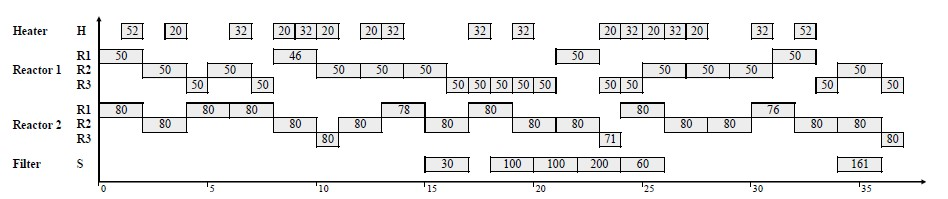
\includegraphics[width=1.0\textwidth]{диаграмма ганта}
\label{fig:gannt_example}
\end{figure}

\section{Модели}
\subsection{Базовая модель с дискретным временем}
\label{subsection:base}

Для начала опишем ещё одну классификацию рассматриваемых моделей. Как было описано ранее, от алгоритма ожидаются ответы на два основных вопроса: Когда запускать задачи на узлах и какое количество вещества подавать на вход. Размер пакета кодируется достаточно просто --- это переменная непрерывного типа (нет требования на целочисленность). О времени есть два основных подхода, хорошо описанные в [reallife]: моделирование \textbf{порядка} запусков на узлах и моделирование фиксированного \textbf{времени} начала запуска. Говоря формально, в первом случае вводятся переменные-индикаторы того, что один процесс начинается раньше другого, а потом выбираются времена как непрерывные переменные. Во втором случае временная шкала делится на периоды и вводятся переменные-индикаторы того, что процесс начался в заданный момент. После этого выбираются времена, как непрерывные переменные. Помимо этого, можно классифицировать второй тип дальше: считаем ли мы ширину промежутка фиксированной (между точками на шкале проходит одинаковый период времени) или плавающей (длина промежутка или точное значение момента времени --- переменная).

Базовая модель, описываемая в этой части будет принадлежать второму типу: мы поделим заранее шкалу на моменты времени и введём переменные для каждого запуска в каждый момент времени. Эта модель взята из [lpheuristic] и критикуется за большое число переменных в случае плотной временной сетки и низкое качество в случае разряженной.

Опишем переменные детальнее: 

\begin{enumerate}

\item $MS$ --- общее время работы системы.
\item $b_{u,j,t}$ --- общее количество вещества, потребряемого процессом $j \in J$ на узле $u \in U$ в момент времени $t \in T$, где $T$ --- натуральные числа некоторого отрезка (времена на шкале). Заранее подбирается константа, являющаяся некоторой оценкой на общее время работы.
\item $s_{p, t}$ --- количество вещества $p \in P$ на складе в момент времени $t \in T$. Считается, что $s_{p, 0}$ даны (начальное состояние складов).
\item $x_{u, j, t}$ --- индикатор того, что задача $j \in J$ началась на узле $u \in U$ в момент времени $t \in T$.

\end{enumerate}

Опишем ограничения:

\begin{enumerate}
	\item $MS \geq x_{u, j, t}t + \Tau_{u, j} \: \forall u \in U, j \in J, t \in T$ --- общее время работы не меньше, чем время окончания каждого процесса.
	\item $x_{u, j, t}B^{min}_u \leq b_{u, j, t} \leq x_{u, j, t}B^{max}_u \: \forall u \in U, j \in J, t \in T$ --- пакет, потребляемый процессом $j \in J$ на узле $u \in U$ лежит между максимальным и минимальным размерами, которые узел может принять. Если процесс не запускается, то вещества он не потребляет.
	\item $s_{p, t} = s_{p, t-1} + \displaystyle\sum_{j \in J^{out}_p, u \in U_j, t - \Tau_{u, j} \geq 1} \mathcal{Q}^{out}_{p, j}b_{u, j, t} - \displaystyle\sum_{j \in J^{in}_p, u \in U_j, t \geq 1} \mathcal{Q}^{in}_{p, j}b_{u, j, t} \; \forall t \geq 1, p \in P$ --- уравнения баланса склада. Количество вещества в момент времени $t$ есть количество вещества в момент $t-1$ плюс то, что успели к этому моменту произвести, минус количество, которое потребляют начатые процессы.
	\item $0 \leq s_{p, t} \leq S^{max}_p$ --- ограничения на объем хранящихся на складе веществ.
	\item $\displaystyle\sum_{j \in U_j, t^{'} \in [t-\Tau_{u, j}, t] x_{u, j, t'}} \leq 1 \; \forall t \in T, u \in U$ --- ограничения одновременности. В момент времени $t$ узел $u$ выполняет не более одной задачи.
	\item $s_{p, 0} = I_p \; \forall p \in P$ --- начальное состояние складов.
	\item $s_{p, max(T)} \geq D_p \; \forall p \in P$ --- требование на заказ.
\end{enumerate}

При использовании этого подхода к процессу, изображенному на диаграмме \ref{fig:stn_exmp} и данных, описанных в \cite{discretetime} было получено 20860 решающих переменных. За 10 минут работы было найдено расписание, затрачивающее 60 рабочих часов, что уступает почти в 2 раза результатам, полученным в оригинальной работе \cite{discretetime}.

\subsection{Двухступенчатая схема.}

Основная проблема базового подхода к моделированию состоит в том, что из-за плотной шкалы времени число переменных становится очень большим. Также сложность получаемых моделей растет не от количества запусков задач на производственных узлах, а преимущественно от их длительности (так как увеличивается количество точек на шкале). Это делает модель абсолютно неприменимой в случае, если makespan растёт.

Однако для того, чтобы записать уравнения баланса склада, которые представляют основное ограничения на запуски процессов, достаточно знать не точное время запуска, а порядок запусков. Это наводит на мысль о том, что можно разрядить временную сетку, позволив системе очень грубо расставить задачи на временной шкале. Очевидно, этот подход даст расписание малого качества, так как задачам станет запрещено запускаться в произвольное время. Однако, получив приближенное расписание, можно решить задачу оптимизации на второй фазе и, зная размеры пакетов всех задач постараться разместить задачи максимально плотно, чтобы минимизировать общее время производства. Более детально этот метод моделирования описан в оригинальной статье \cite{lpheuristic}, в которой он был впервые предложен.

Первая фаза совпадает с базовой моделью с дискретным временем из ~\ref{subsection:base}. Единственное отличие, что теперь множество временных меток $T$ содержит не всевозможные времена начала задачи, а только некоторые (например, кратные некоторому значению). \textbf{Шириной} временной сетки будем называть расстояние между соседними точками (подразумевается, что оно одинаковое). Заметим, что если взять ширину сетки равной максимальному времени, то задача составления расписания упрощается, так как на одной машине при любом выборе времени начала задачи сами задачи не пересекутся во времени. Это позволяет не писать отдельно ограничения. Выбор ширины сетки представляет собой отдельную исследовательскую задачу, так как ведёт к упрощению модели, но ухудшению качества расписания. Это явление в английской литературе называется <<tradeoff>>.

На второй фазе ставится задача оптимизации, однако размеры пакетов для задач считаются известными, что упрощает модель. Также грубое приближение даёт некоторые ограничения на максимальные и минимальные значения времени старта и окончания задачи.

Переменные:

\begin{enumerate}

\item $MS$ --- общее время работы системы.
\item $S_{n, u}, F_{n, u}$ --- минимальные времена старта и окончания $n$-той задачи, работающей на узле $u \in U$. В отличие от первой фазы, тут задачи не делятся по типу, так как тип задачи уже не важен. В первой фазе алгоритм определил задачи и их последовательность, а так же потребляемые материалы, а значит теперь необходимо их просто плотнее поставить на шкале. Значит, решающих переменных стало меньше
\item $s_{n, u, t}, f_{n, u, t}$ --- <<переменные Хевисайда>>, индикаторы того, что $S_{n, u} \leq t$ и $F_{n, u} \leq t$. На сей раз $t$ берется не из разряженной шкалы, а из полной. Эти переменные требуются для описания баланса склада --- для момента времени $t$ можно выразить всё, что на склад было отправлено как произведение размера пакета операции на индикатор того, что операция успела начаться, а так же всё, что с склада было извлечено.
\item $stock_{p, t}$ --- объем вещества на складе к моменту времени $t$.

\end{enumerate}

Будем обозначать $\overline S_{n, u}, \underline S_{n, u}$ --- верхняя и нижняя границы на время начала. Аналогичные ограничения можно ввести на время окончания. Верхней границей на время начала окончания будет полученное время на первой фазе: цель второй фазы состоит в том, что алгоритм распологает плотнее задачи на шкале. Очевидно, ожидается, что новое время начала будет меньше предыдущего. Нижняя граница считается тривиально: $\underline S_{n, u} = \displaystyle\sum_{m < n} \Tau_{u, j_m}$ --- сумма времён выполнения всех предыдущих задач. $\underline T_{n, u} = \underline S_{n, u} + \Tau_{u, j_n}$ --- нижняя граница на время окончания задачи получается из границы на время старта прибавлением длительности задачи.

Ограничения:

\begin{enumerate}
	\item $MS \geq F_{u, n}$ --- общее время работы не меньше, чем время окончания каждого процесса.
	\item $S_{n, u} \geq F_{n-1, u}$ --- очередная задача начинается не раньше, чем закончится предыдущая.
	\item $F_{n, u} = S_{n, u} + \Tau_{u, j_n}$ --- время окончания это время начала плюс длительность задачи.
	\item $s_{n, u, t} \leq \frac{t - S_{n, u}}{max(T)} + 1$, $s_{n, u, t} \geq \frac{t - S_{n, u} + 1}{max(T)}$, $f_{n, u, t} \leq \frac{t - F_{n, u}}{max(T)} + 1$, $f_{n, u, t} \geq \frac{t - F_{n, u} + 1}{max(T)}$ --- <<переменные Хевисайда>> действительно являются индикаторами того, событие начала и конца выполнения задачи произошло не раньше некоторого времени. $max(T)$ --- максимальное рассматриваемое время.
	\item $s_{n, u, t} = 0$ при $t < \underline S_{n, u}$ и $s_{n, u, t} = 1$ при $t \geq \overline S_{n, u}$. $f_{n, u, t} = 0$ при $t < \underline F_{n, u}$ и $f_{n, u, t} = 1$ при $t \geq \overline F_{n, u}$ --- ограничения на минимальное и максимальное время старта и окончания, описанное выше.
	\item $stock_{p, t} = s_{p, 0} + \displaystyle\sum_{u \in U, n \in N_u}  q^{out}_{u, n, p} f_{n, u, t} - q^{in}_{u, n, p} s_{n, u, t}$, где $q^{in}_{u, n, p}, q^{out}_{u, n, p}$ --- потребляемое и производимое количество материала $n$-той операцией, производимой на узле $u$. Эти величины можно посчитать, используя размеры пакетов $b_{u, j, t}$, посчитанные в первой фазе. Для этого следует выбрать те моменты времени $t$, когда задача действительно была запущена (пакет имеет ненулевой размер), отсортировать пакеты по времени и назначить номера задачам, а также умножить размер пакета на $\mathcal{Q}^{in}_{p, j}$ или $\mathcal{Q}^{out}_{p, j}$ --- долю содержания в нём нужного вещества.
	\item $stock_{p, max(T)} \geq D_p$ --- требование на заказ.
\end{enumerate}

Основной выигрыш данного подхода состоит в разбиении задачи составления на две подзадачи: определение примерного порядка и размера пакета для каждой задачи и уточнение времён запуска для достижения оптимальности. Именно из-за использования на втором этапе грубого приближения из первого теряется оптимальность расписания.

\section{Заключение}
Желательно, чтобы этот раздел был, причём он не~должен дословно повторять аннотацию.
Обычно здесь отмечают, каких результатов удалось добиться, какие проблемы остались открытыми.

%%%% если имеется doi цитируемого источника, необходимо его указать, см. пример в \bibitem{article}
%%%% DOI публикации, зарегистрированной в системе Crossref, можно получить по адресу http://www.crossref.org/guestquery/
\begin{thebibliography}{99}

\bibitem{lpheuristic}
    \BibAuthor{F. Blomer, H.-O. Gunther}
    LP-based heuristics for scheduling chemical batch processes, 2010
    \BibJournal{International Journal of Production Research}, 38:5, 1029-1051
	\BibDoi{10.1080/002075400189004}.

\bibitem{dairy}
    \BibAuthor{Georgios P. Georgiadis, Georgios M. Kopanos, Antonis Karkaris, Harris Ksafopoulos and Michael C. Georgiadis}
    Optimal Production Scheduling in the Dairy Industries, 2019
    \BibJournal{Industrial \& Engineering Chemistry Research} 58 (16), 6537-6550
	\BibDoi{10.1021/acs.iecr.8b05710}.
	
\bibitem{reallife}
    \BibAuthor{Georgiadis, Georgios P. and Elekidis, Apostolos P. and Georgiadis, Michael C.}
    Optimization-Based Scheduling for the Process Industries: From Theory to Real-Life Industrial Applications, 2019
    \BibJournal{Industrial \& Engineering Chemistry Research} 58 (16), 6537-6550
	\BibDoi{10.3390/pr7070438}.
	
\bibitem{hybridizing}
    \BibAuthor{Siqun Wang, Monique Guignard}
    Hybridizing Discrete- and Continuous-Time Models For Batch Sizing and
Scheduling Problems, 2006
    \BibJournal{Computers \& Operations Research} Volume 33, Issue 4
	\BibDoi{10.1016/j.cor.2004.11.013}.
	
\bibitem{discretetime}
    \BibAuthor{Christos T. Maravelias and Ignacio E. Grossmann}
    Minimization of the Makespan with a Discrete-Time State-Task Network Formulation, 2003
    \BibJournal{Industrial \& Engineering Chemistry Research}
	\BibDoi{10.1021/ie034053b}.
	
\bibitem{stnoriginal}
    \BibAuthor{E.Kondili, C.C.Pantelides, R.W.H.Sargent}
    A general algorithm for short-term scheduling of batch operations—I. MILP formulation, 1993
    \BibJournal{Computers \& Chemical Engineering}
	\BibDoi{10.1021/ie034053b10.1016/0098-1354(93)80015-F}.
	
%\bibitem{webArticle}
%	\BibAuthor{Blaga~P.\,A.}
%	Commutative Diagrams with XY-pic II. Frames and Matrices~//
%	\BibJournal{PracTEX J.}, 2007. Vol.\,4.
%	URL: \BibUrl{https://tug.org/pracjourn/2007-1/blaga/blaga.pdf}.
%
%\bibitem{webResource}
%	XYpic.
%	URL: \BibUrl{http://akagi.ms.u-tokyo.ac.jp/input9.pdf}.
%	
%\bibitem{inproceedingsRus}
%	\BibAuthor{Усманов~Т.\,С., Гусманов~А.\,А., Муллагалин~И.\,З., Мухаметшина~Р.5\,Ю., Червякова~А.\,Н., Свешников~А.\,В.}
%	Особенности проектирования разработки месторождений с применением гидроразрыва пласта~//
%	\BibJournal{Труды 6-го Междунар. симп. <<Новые ресурсосберегающие технологии недропользования и повышения нефтегазоотдачи>>}.~---
%	М.:~Издательство, 2007. С.~267--272.

%\bibitem{inproceedingsEng}
 %   \BibAuthor{Author~N.}
  %  Paper title~//
   % \BibJournal{10th Conference (International) on Any Science Proceedings}.~---
    %Place of publication: Publisher, 2009. P.~111--122.

%\bibitem{techreport}
%	\BibAuthor{Lambert~P.}
 % 	\BibTitle{The title of the work}.
  %	Place of publication:~The institution that published, 1993.  Report~2.
 	
\end{thebibliography}

%%%% если имеется doi цитируемого источника, необходимо его указать, см. пример в \bibitem{article}
%%%% DOI публикации, зарегистрированной в системе Crossref, можно получить по адресу http://www.crossref.org/guestquery/.

\end{document}
